\section{Experiments}

% \begin{frame}{Experiments}
%   \textbf{Dataset: MS--COCO 2014}
%   \begin{itemize}
%     \item 82 k train / 40 k val images, 80 object categories.
%     \item Avg. 2.9 labels / image.
%     \item Single-positive variant generated for MLSPL.
%   \end{itemize}
% \end{frame}

% %-------------------------------------------------

% \begin{frame}{Experiments}
%   \begin{itemize}
%     \item Reproduced authors' pipelines under 12 GB GPU budget.
%     \item Hyper-parameter grid: $\text{LR}\in[10^{-2},10^{-5}],\;\text{batch}\in\{8,16\}.$
%     \item MLSPL: linear classifier then fine-tuning.
%   \end{itemize}
% \end{frame}

% %-------------------------------------------------



% --- Slide: Experimental Setup ---
\begin{frame}{Experiments}
  \begin{itemize}
  \item \textbf{Hardware:} 2$\,\times$ NVIDIA RTX 3060 GPUs (12 GB VRAM) on Ubuntu 22.04.5 LTS.

  \item \textbf{Q2L Environment:}
    \begin{itemize}
      \item Python~3.7.3, PyTorch~1.9.0, Torchvision~0.10.0, CUDA~11.1.
      \item \texttt{inplace\_abn} rebuilt from earlier release for compatibility.
      \item \textbf{RandAugment dependency missing:}
        \begin{itemize}
          \item Added local \texttt{augmentations.py} from \textit{pytorch-randaugment}.
          \item Changed import in \texttt{get\_dataset.py}: \texttt{from .augmentations import RandAugment}.
          \item Replaced default call with \texttt{RandAugment(n=2, m=9)} to set parameters explicitly.
        \end{itemize}
    \end{itemize}

  \item \textbf{MLSPL Environment:}
    \begin{itemize}
      \item Python~3.11.8, PyTorch~2.2.1, Torchvision~0.17.1, CUDA~12.4.
      \item Single-GPU training to ensure reproducibility across runs.
    \end{itemize}
\end{itemize}
% \begin{itemize}
%   \item \textbf{Hardware:} 2\,$\times$ NVIDIA RTX 3060 GPUs (12 GB VRAM) on Ubuntu 22.04.5 LTS.
%   \item \textbf{Q2L:}
%     \begin{itemize}
%       \item Python~3.7.3, PyTorch~1.9.0, Torchvision~0.10.0, CUDA~11.1.
%       \item \texttt{inplace\_abn} rebuilt from earlier release due to compatibility issues.
%       \item Manually added \texttt{augmentations.py} from 
%     \end{itemize}
%   \item \textbf{MLSPL:}
%       \begin{itemize}
%         \item Python~3.11.8, PyTorch~2.2.1, CUDA~12.4.
%         \item Single-GPU training to ensure reproducibility.
%       \end{itemize}
% \end{itemize} 
\end{frame}

% --- Slide: Dataset & Metric ---
\begin{frame}{Experiments}
\begin{columns}
  \begin{column}{0.55\textwidth}
    \textbf{Dataset: MS-COCO 2014}
    \begin{itemize}
      \item 82,081 training images
      \item 40,137 validation images.
      \item 80 categories - multiple objects per image.
    \end{itemize}
    \vspace{0.4em}
    \textbf{Metric: mean Average Precision (mAP)}
    \begin{itemize}
      \item Widely reported metric in MLC.
      \item Used in both Q2L and MLSPL.
    \end{itemize}
  \end{column}
  \begin{column}{0.4\textwidth}
        \begin{figure}[b]
        \centering
        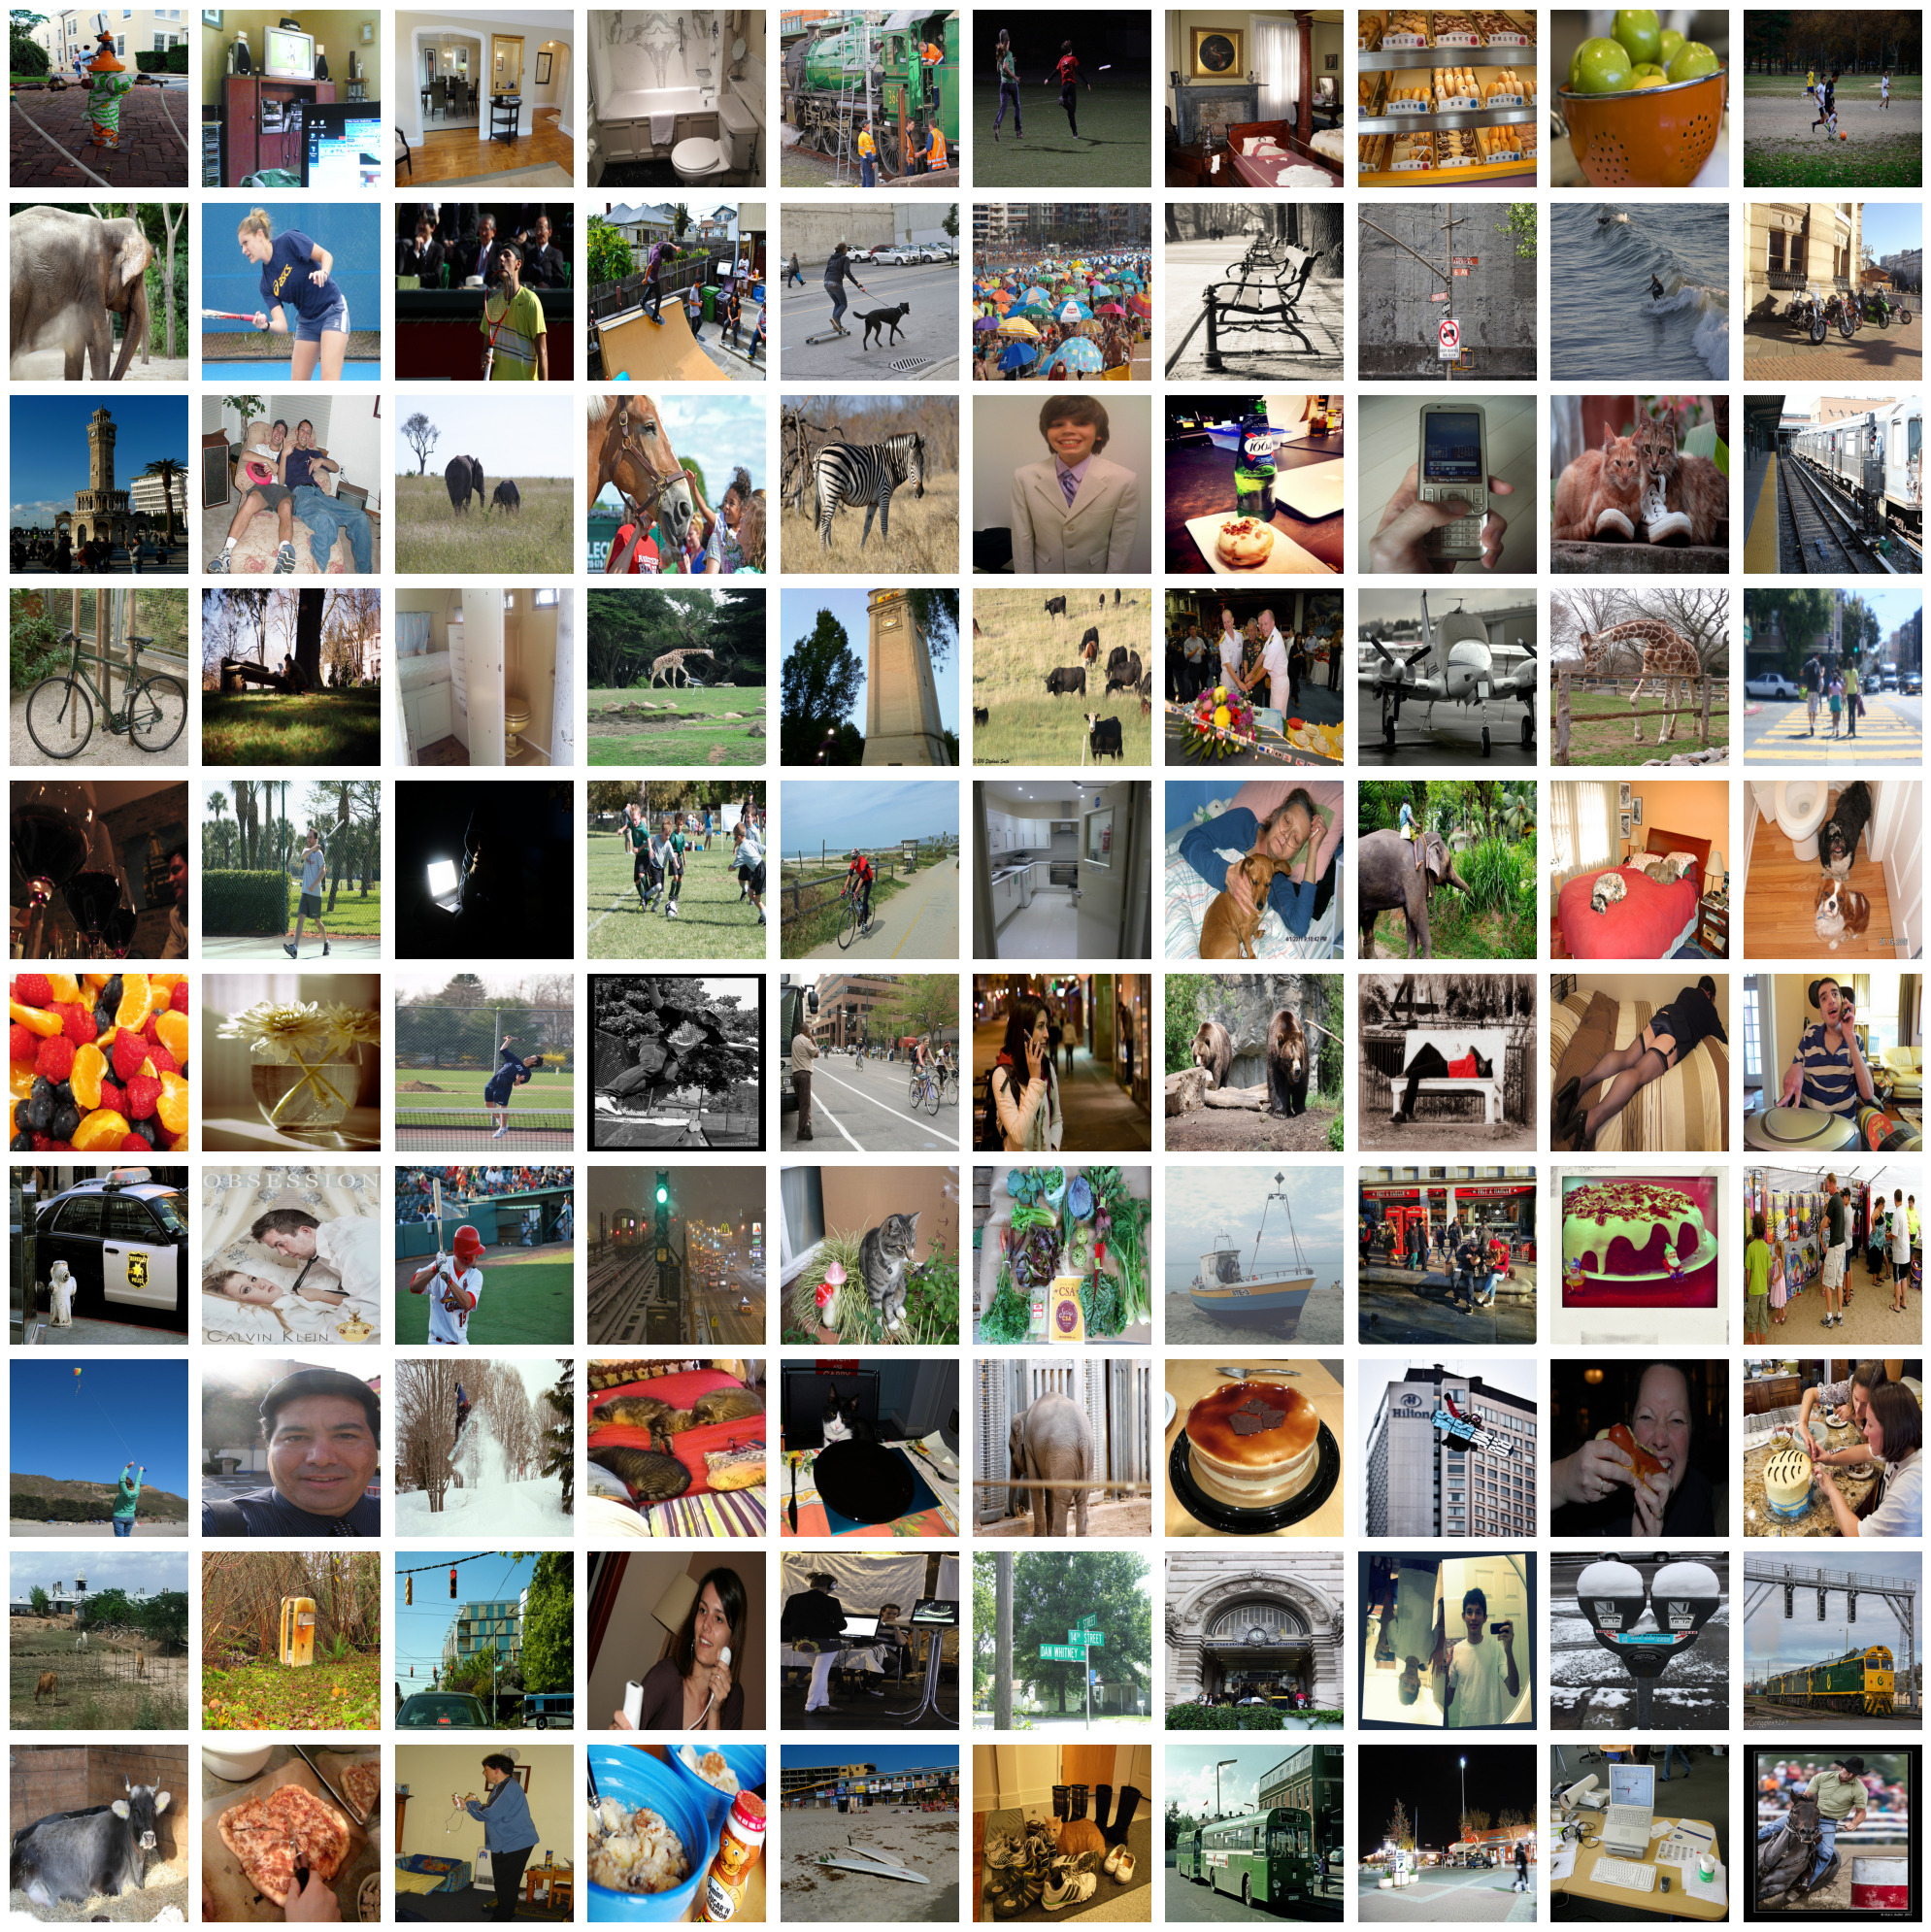
\includegraphics[width=0.9\linewidth]{Images/coco_examples.png}
        \caption*{\tiny Example COCO images (448$\times$448)}
    \end{figure}
  \end{column}
\end{columns}
\end{frame}

% --- Slide: Query2Label Experiments ---
\begin{frame}{Experiments}
  \textbf{Q2L}
\textbf{Backbones evaluated}
\begin{itemize}
  \item ResNet-101: 448 and 576
  \item TResNetL 448
  \item TresNetL (22k) 448
  \item Swin-L (22k) 384
  \item CvT-w24 (22k) 384
\end{itemize}
\textbf{Training protocol}
\begin{itemize}
  \item Pre-trained weights from authors - batch size 16.
  \item Scratch training attempted with all backbones.
  \item Memory overflow with SwinL and CvT-w24 during training.
\end{itemize}
\end{frame}



% --- Slide: MLSPL Experiments ---
\begin{frame}{Experiments}
\textbf{MLSPL Experiments}
\begin{itemize}
  \item Convert each image to exactly one positive label.
  \item \textit{Linear} classifier on fixed features (25 epochs).
  \item End-to-end \textit{fine-tuning} (10 epochs).
\end{itemize}
\textbf{Hyperparameter search}
\begin{itemize}
  \item Learning rate \(\in\{10^{-2},10^{-3},10^{-4},10^{-5}\}\).
  \item Batch size \(\in\{8,16\}\).
\end{itemize}
\textbf{Selected configuration}
\begin{itemize}
  \item \textbf{Linear}: lr = \(10^{-3}\), batchsize 16.
  \item \textbf{Fine-tuned}: lr = \(10^{-5}\), batchsize 16.
\end{itemize}
\end{frame}

